\chapter[Deserción en Chile]{Deserción en Chile}
\label{ch:tema}


\section{Deserción en Chile}
\label{sec:deserción}

En los últimos 30 años en Chile ha existido un crecimiento de manera significativo en el número de matrículas de pregrado para la educación superior, de 165 mil estudiantes matriculados a principios de los ochenta, a más de un millón de estudiantes para el año 2012.\\

El cual ha marcado un gran cambio en el sistema de educación superior, pasó de ser un sistema de élite a uno masivo. Sin embargo, este cambio trajo consigo el aumento de diferentes problemas, como es el caso de la deserción.\\

La deserción no es un fenómeno aislado, las cifras en porcentaje son muy elevadas, aproximadamente un 50 \% de los alumnos que entran a universidades o centros de formación técnica no terminan su programa de estudio al cual se matricularon, situación que preocupa tanto al Estado como a los distintos actores del sistema. El Estado pierde recursos, los estudiantes y sus familias pierden la inversión en la formación de quienes no completan sus estudios, las instituciones se ven afectadas ya que dejan de recibir recursos asociados a estos estudiantes y deben adaptar su funcionamiento en cursos superiores a un menor número de alumnos. Además, para los jóvenes que desertan sus sueños de graduarse se estancan, lo que les genera frustración y descontento.\\


\subsection{Estadísticas de deserción en Chile}

En Chile desde el año 2006 surge el Servicio de Información de Educación Superior (SIES), del Ministerio de Educación, a través del mandato establecido en la Ley 20.129, la que en su artículo 49 \textsuperscript{\underline{o}} señala ``corresponderá al Ministerio de Educación, a través de su División de Educación Superior, desarrollar y mantener un Sistema Nacional de Información de la Educación Superior, que contenga antecedentes necesarios para la adecuada aplicación de las políticas públicas destinadas al sector de educación superior, para la gestión institucional y la información pública de manera de lograr una amplia y completa transparencia académica, administrativa y contable de las instituciones de educación superior'' \cite{sies}. \\

El SIES recopila datos de las matriculas de prácticamente la totalidad de las instituciones de educación superior, con los cuales genera informes anuales de las tasas de retención. La retención se es la contraparte de la deserción, indica cuántos alumnos siguen sus estudios y logran continuar a la obtención de su título. El documento más reciente sobre las tasas de retención de las instituciones abarca los años 2010 al 2014 y se puede ubicar en \cite{Sies2014}. Dicho documento, operacionalmente, calcula la tasa de retención al primer año como el cociente entre el número de estudiantes que ingresan como alumnos de primer año a un programa de estudios en un año determinado y el número de estos mismos estudiantes que se mantienen como estudiantes antiguos en la misma institución al año siguiente.\\

A continuación, se presentará una serie de estadísticas que describen el comportamiento de la retención entre los años 2010 y el año 2014.\\

\begin{figure}[H]
	\centering 
	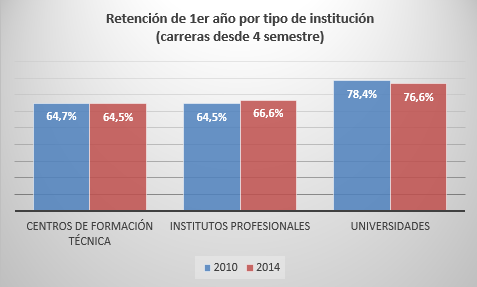
\includegraphics[width=10cm,height=5cm] {retencioninstituciones.png} 
	\caption{Retención de 1er año por Tipo de Institución} \label{fig:institucion}
\end{figure}

En la Figura \ref{fig:institucion} se puede apreciar la evolución de la retención en las instituciones chilenas entre los años 2010 y 2014. En el año 2014 la retención, tanto el CFT como en Universidades bajó con respecto al año 2010, la disminución se distribuye en un 0,2 \% para CFT, y de un 1,8 \% para Universidades, mientras que los Institutos registraron un alza de 2,1 \%. \\

\begin{figure}[h]
	\centering 
	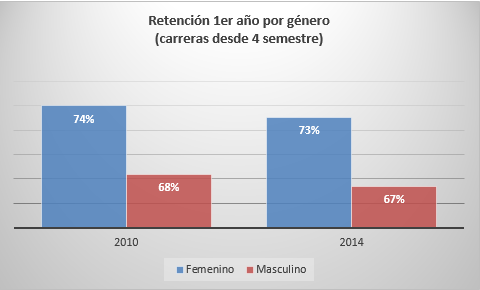
\includegraphics[width=10cm,height=5cm] {retenciongenero.png} 
	\caption{Retención de 1er año por Género} \label{fig:genero}
\end{figure}


En cuanto a género la evolución de la tasa de deserción se puede apreciar en la Figura \ref{fig:genero}, donde para ambos género ha existido una baja en la tasa de retención, para el año 2010 se registra un 74 \% para el género femenino y un 68 \% para el género masculino, y para el año 2014 se registra un 73 \% para el género femenino, y un 67 \% para el género masculino, ambos con una baja de 1 \%.\\  

\begin{figure}[H]
	\centering 
	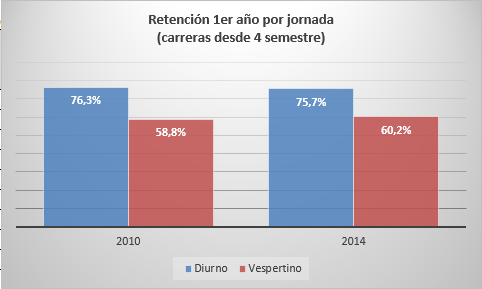
\includegraphics[width=10cm,height=5cm] {retencionjornada.png} 
	\caption{Retención de 1er año por Jornada} \label{fig:jornada}
\end{figure}

En lo que respecta a las jornadas de estudios, para el año 2010 la tasa de retención para carreras diurnas fue del 76,3 \% y para carreras vespertinas fue de un 58,8 \%, mientras que para el año 2014, para la jornada diurna fue de 75,7 \% teniendo una baja de 0.6 \%, y para la jornada vespertina, fue de 60,2 \% obteniendo un incremento de 1,4 \%, ver Figura \ref{fig:jornada}.\\

\begin{figure}[h]
	\centering 
	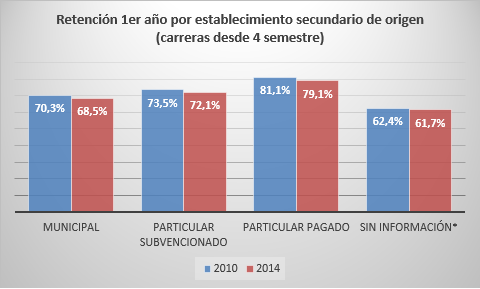
\includegraphics[width=10cm,height=5cm] {retencionestablecimiento.png} 
	\caption{Retención de 1er año por Establecimiento de Origen} \label{fig:establecimiento}
\end{figure}


La Figura \ref{fig:establecimiento}, genera la estadística a partir de los establecimientos de origen de los alumnos, mostrando para el año 2010 los siguientes resultados. Para establecimientos municipales un 70,3 \%, para establecimientos particular subvencionado un 73,5 \%, para establecimientos particular pagado un 81,1 \% y para establecimientos sin información (matricula sin información de colegio de origen) un 62,4 \%. Para el año 2014, para establecimientos municipales hubo una baja de 1,8 \%, marcando 68,5 \%, para establecimientos particular subvencionado hubo una baja de 1,4 \%, marcando 72.1 \%, para establecimientos particular pagado hubo una baja de 2 \%, marcando 79.1 \%, para establecimientos sin información, también hubo una baja de 0,7 \%, marcando 61.7 \%.  \\

\begin{figure}[h]
	\centering 
	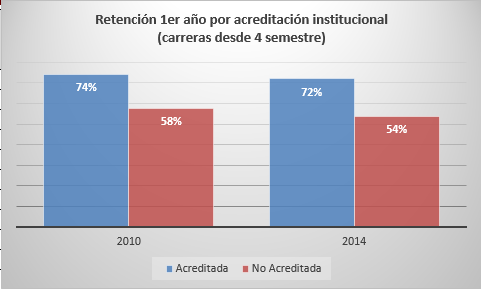
\includegraphics[width=10cm,height=5cm] {retencionacreditacion.png}
	\caption{Retención de 1er año por Acreditación Institucional} \label{fig:acreditacion}
\end{figure}

La estadística para instituciones con y sin acreditación se puede visualizar en la Figura \ref{fig:acreditacion}, mostrando para el año 2010, para instituciones acreditadas un 74 \% y para instituciones no acreditadas un 58 \%. Para el año 2014, para instituciones acreditadas hubo una baja del 2 \%, marcando 72 \%, para las instituciones no acreditadas hubo una baja del 4 \%, marcando 54 \%.\\   



Las estadísticas presentadas anteriormente muestran un análisis del comportamiento entre los años 2010 y 2014, a partir de variables como lo es la institución, el género, la jornada, el establecimiento de origen y la acreditación de las instituciones